
\section{Theoretical Uncertainties}
\label{sec:TheoSystematics}

\indent Theoretical uncertainties quantify the uncertainty associated with MC generation including different scale parameters such as QCD renormalization, factorization scales and calculations on the matrix element and parton shower.  We vary MC generation with respect to the default setting and get different MC yields in the control and signal regions.  Because the background rate is normalized to the data in the control region, only differences in the transfer factor (defined in equation \ref{eqn:TF}) will result in a different signal region background prediction.    \\

\begin{equation}
T = \frac{N_{MC}^{SR}}{N_{MC}^{CR}}
\label{eqn:TF}
\end{equation}

\indent $N_{MC}^{SR}$ is the MC yield in the signal region and $N_{MC}^{CR}$ is the MC yield in the control region. \\

\indent  We determine the variation in the signal region background prediction according to the variation in the transfer factor as defined in equation \ref{eq:theory_uncertainty}.   All theoretical uncertainties for different backgrounds are assumed to be independent of one another.  \\

 \begin{eqnarray}
    \Delta_{X} = \frac{T_f^{\mathrm{up}} - T_f^{\mathrm{down}}}{T_f^{\mathrm{up}} + T_f^{\mathrm{down}}}
    \label{eq:theory_uncertainty}
  \end{eqnarray}

\indent $T_f^{\mathrm{up}}$ ($T_f^{\mathrm{down}}$) is the transfer factor defined in equation \ref{eqn:TF} for the upward (downward) variation in the systematics and $\Delta_{X}$ is the uncertainty due to parameter $X$ in the signal region.  \\

\subsection{$\ttbar$ Theoretical Uncertainty}
\label{sec:systTheo:ttbar}

\indent Theoretical uncertainties on $\ttbar$ production include uncertainties on the hard scattering matrix element calculation, uncertainties on the parton shower, and uncertainty on the amount of ISR/FSR produced in association with $\ttbar$.  \\

%\indent The $\ttbar$ ISR/FSR uncertainty is estimated by performing the analysis on fully reconstructed simulation with variations on the PS tuning and ME+PS matching scales that induces more/less ISR and FSR in the simulation. 

\indent  The $\ttbar$ ISR/FSR uncertainty is estimated by producing $\powheg\pythia$ MC samples with a different amount of radiation than the nominal MC sample.  These ISR/FSR variation samples are called the radHi and radLo samples.  In general, the radHi (radLo) sample generates a higher (lower) differential cross-section for $\ttbar$ that is produced in conjunction with hard ISR. \\

\indent The radHi and radLo samples are produced with different renormalization and factorization scales compared to the nominal sample (x0.5 to radHi and x2 to radLo).   The radHi sample also increase the $h_{damp}$ parameter which controls the matching between the parton shower and matrix element calculations.  The $h_{damp}$ parameter is increased from the nominal $m_{t}$ to $2 \times m_{t}$ for the radHi sample.   \\

\indent The $\ttbar$ ISR/FSR uncertainty ($ \Delta_{\ttbar ISR/FSR} $) is estimated using equation \ref{eq:ttbar_ISRuncert} where $T_f^{\mathrm{radHi}}$ ($T_f^{\mathrm{radLo}}$) is the transfer factor corresponding to the radHi (radLo) sample. \\

\begin{eqnarray}
    \Delta_{\ttbar ISR/FSR} = \frac{T_f^{\mathrm{radHi}} - T_f^{\mathrm{radLo}}}{T_f^{\mathrm{radHi}} + T_f^{\mathrm{radLo}}}
    \label{eq:ttbar_ISRuncert}
\end{eqnarray}

%\indent The uncertainty on the ME calculation and on the PS calculation is estimated by performing the analysis on truth level-simulation using different MC generator programs.  In short, the ISR/FSR uncertainty determines how much the $\ttbar$ yields in the signal region differ if different $\powheg$ and $\pythia$ settings were used.  The $\ttbar$ hard scattering and PS variations determines how much the $\ttbar$ yields in the signal region differ if different generator programs and parton shower tunes are used. \\

\indent Uncertainties on the hard scattering and parton shower are calculated by comparing the nominal $\powheg\pythia$ $\ttbar$ sample with the $\powheg\herwigpp$ $\ttbar$ and $\sherpa$ 2.2.1 $\ttbar$ samples.  The $\powheg\herwigpp$ sample has the same matrix element calculation as the nominal sample but uses $\herwigpp$ to perform a different set of parton shower calculation with a distinct parton shower tune.  The $\sherpa$ 2.2.1 $\ttbar$ sample perform a different matrix element and parton shower calculation using a different PDF set and parton shower tune.  More details on the different $\ttbar$ MC generation can be found in section \ref{sec:MC:Bkg}. \\

\indent We take an envelope of the $\sherpa$ and $\powheg\herwigpp$ variations as the combined $\ttbar$ hard scattering and parton shower uncertainty.  This is because the $\powheg\herwigpp$ and $\sherpa$ samples both vary the parton shower calculations.  Taking an envelope of both variations instead of summing the two in quadrature avoids double counting the parton shower uncertainty. The total hard scattering plus parton shower uncertainty is defined as the maximum of equation \ref{eq:ttbar_ME_uncertainty} and \ref{eq:ttbar_PS_uncertainty}.  \\

    \begin{eqnarray}
      \Delta_{\mathrm{hard~scatter}} = \frac{T_f^{\mathrm{\powheg\pythia}} - T_f^{\mathrm{\sherpa}}}{T_f^{\mathrm{\powheg\pythia}}}
      \label{eq:ttbar_ME_uncertainty}
    \end{eqnarray}

    \begin{eqnarray}
      \Delta_{\mathrm{PS}} = \frac{T_f^{\mathrm{\powheg\pythia}} - T_f^{\mathrm{\powheg\herwigpp}}}{T_f^{\mathrm{\powheg\pythia}}}
      \label{eq:ttbar_PS_uncertainty}
    \end{eqnarray}

\indent $T_f^{\mathrm{\powheg\pythia}}$, $T_f^{\mathrm{\powheg\herwigpp}}$ and $T_f^{\mathrm{\sherpa}}$ correspond to the transfer factors derived by using the nominal $\powheg\pythia$ $\ttbar$ MC, the $\powheg\herwigpp$ $\ttbar$ MC and the $\sherpa$ $\ttbar$ MC.  $\Delta_{\mathrm{hard~scatter}}$ is the uncertainty on the hard scattering calculation and $\Delta_{\mathrm{PS}}$ is the uncertainty on the parton shower calculation. \\

\indent The MC $\ttbar$ yields in the control region, validation region and signal region for the different $\ttbar$ samples and the $\ttbar$ theory uncertainties are given in Table \ref{tab:ttbar_unc_SRC}  \\

\pagebreak
  
 \begin{table}[!h]
    \begin{center} \footnotesize
    
        \begin{tabular}{|c|c|c|c|c|}
	\noalign{\smallskip}\noalign{\smallskip}\hline
        & CRTopC & VRTopC & SRC1 & SRC2\\
        \hline
$\ttbar$ (nominal)&   $668\pm 9 $&         $232\pm 5 $ &    $16.7\pm 1.6 $&         $31.7\pm 2.1 $\\
$\ttbar$ (rad up)&          $872\pm 11 $&         $293\pm 7 $ &            $25.2\pm 2.3 $&         $39.5\pm 2.3 $\\
$\ttbar$ (rad down)&        $521\pm 9 $&   $187\pm 5 $ &         $10.1\pm 1.0 $&         $19.2\pm 1.6 $\\
$\ttbar$ (Powheg+H++)&      $621\pm 10 $&         $206\pm 5 $&      $16.3\pm 1.8 $&         $27.8\pm 1.8 $\\
%$\ttbar$ (aMC@NLO+P8)&      $310\pm 60 $&          $113\pm 34 $&       $6\pm 5 $&      $<0.01$\\
$\ttbar$ (Sherpa)&          $840\pm 40 $&        $297\pm 30 $&            $30\pm 8 $&     $42\pm 9 $\\        
        \hline
        \multicolumn{3}{c}{\bf Transfer factors (in \%)} \\ \hline
        ISR/FSR &  &    $3.3$&      $20$&   $10$\\
        PS &     &   $4$&   $5$&    $6$\\
%        Generator (aMC@NLO) &  &          $46$&     $2$&   $32$\\
        Generator (Sherpa) &    &          $2$&    $40$&   $5$\\
        \hline       
        \end{tabular}
    
      \begin{tabular}{|c|c|c|c|}
	\noalign{\smallskip}\noalign{\smallskip}\hline
          & SRC3 & SRC4 & SRC5 \\
        \hline
$\ttbar$ (nominal) &         $21.7\pm 1.6 $&         $6.3\pm 0.8 $&          $0.60\pm 0.23 $\\
$\ttbar$ (rad up)&         $28.7\pm 2.1 $&         $8.6\pm 1.0 $&  $1.05\pm 0.33 $\\
$\ttbar$ (rad down)&         $15.8\pm 1.5 $&         $6.3\pm 1.2 $&  $0.7\pm 0.4 $\\
$\ttbar$ (Powheg+H++)&         $18.0\pm 1.5 $&         $6.5\pm 0.9 $&  $0.46\pm 0.18 $\\
%$\ttbar$ (aMC@NLO+P8)&        $4\pm 7 $&      $1\pm 5 $&      $0.9\pm 0.9 $\\
$\ttbar$ (Sherpa)&     $22\pm 5 $&     $7.4\pm 3.2 $&          $<0.01$\\        
        \hline
        \multicolumn{4}{c}{\bf Transfer factors (in \%)} \\ \hline
        ISR/FSR  &   $4$&    $10$&   $5$\\
        PS &    $11$&   $11$&   $20$\\
%        Generator (aMC@NLO) &          $15$&   $39$&   $40$\\
        Generator (Sherpa)  &    $19$&   $10$&   $100$\\
        \hline       
        \end{tabular}
       
        
    \end{center}
    \caption{MC yields and theory uncertainties for the $\ttbar$\ background for the control, validation and signal regions.  MC yields are quoted for before any fitting to the data in the control region. Uncertainties are derived using variations in the transfer factor according to equations \ref{eq:ttbar_ISRuncert}, \ref{eq:ttbar_ME_uncertainty} and \ref{eq:ttbar_PS_uncertainty}. The uncertainties are symmetrical and are quantified as percentage of total background yield. }
    \label{tab:ttbar_unc_SRC}
  \end{table}

\subsection{$\Wjets$ Theoretical Uncertainty}

\indent The $\sherpa$ generator is used to estimate $\Wjets$ theory uncertainties.  Variations of the renormalization and factorization scales are included.  The uncertainty for each variation is quantified as the uncertainty on the transfer factor according to equation \ref{eq:theory_uncertainty}.  The total $W$+jets theory uncertainty is the combination of all uncertainties summed in quadrature. \\

\indent The total theory uncertainty on $\Wjets$ in the signal region is given in Table \ref{tab:WThSyst}.  Values are given as percent uncertainties on $\Wjets$ yields in the signal region.  The uncertainties are symmetrical. \\

  \begin{table}[!h]
    \begin{center} \footnotesize
    \begin{tabular}{|c|c|} \hline
{\bf SR} & {\bf uncertainty (\%)} \\ \hline
%SRA-TT & 9.5\\ \hline
%SRA-TW & 8.0\\ \hline
%SRA-T0 & 6.1\\ \hline
%SRB-TT & 9.1\\ \hline
%SRB-TW & 7.9\\ \hline
%SRB-T0 & 3.3\\ \hline
%SRC1 & 11.4\\ \hline
SRC1 & 12.5\\ \hline
SRC2 & 11.8\\ \hline
SRC3 & 10.7\\ \hline
SRC4 & 9.5\\ \hline
SRC5 & 11.3\\ \hline
%SRD-low & 8.8\\ \hline
%SRD-high & 8.2\\ \hline
%SRE & 9.5\\ \hline
%VRW & 1.9\\ \hline
\end{tabular}

    \end{center}
    \caption{Summary of the theory uncertainties (in percent) on $W$ production obtained using variations on transfer factors. The uncertainties are symmetrical and are quantified as percentage of total background yield.}
    \label{tab:WThSyst}
  \end{table}        

\subsection{Single-top Theoretical Uncertainty}

\indent Single-top theoretical uncertainties include the uncertainties on the parton shower, ISR/FSR, and the interference between $\ttbar$ and single-top in the Wt channel.  Single-top uncertainties are evaluated for the $Wt$ subprocess because the $Wt$ subprocess dominates the single-top background in the signal region.  A Feynman diagram for $Wt$ production is given in Figure \ref{fig:ST:feyn}.\\

\begin{figure}[h!]
\begin{center}
	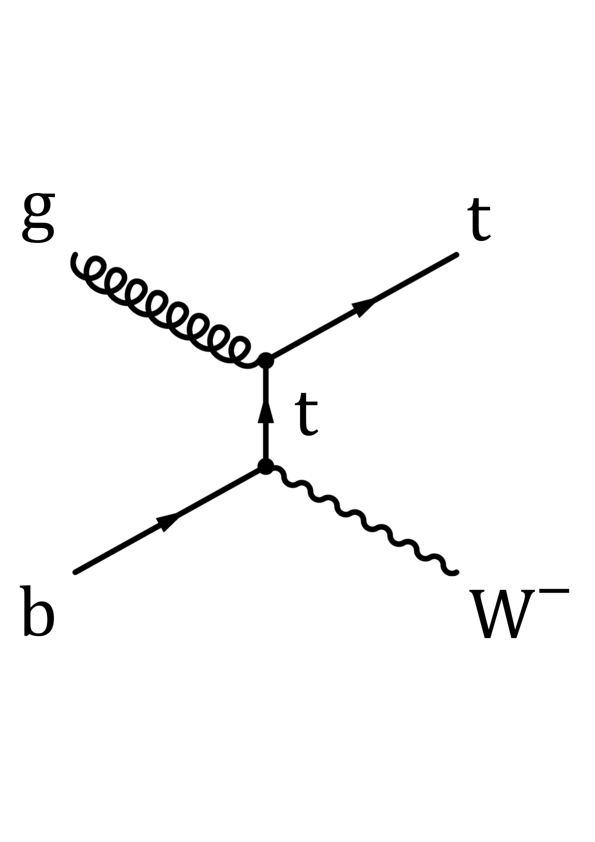
\includegraphics[width=0.45\textwidth]{figures/feynDiag/tW_chan.png}
\end{center}
\caption[Single top production Feynman diagram for the $Wt$ channel.]{Single top production Feynman diagram for the $Wt$ channel. }
\label{fig:ST:feyn}
\end{figure}

\indent The single-top parton shower uncertainty is modeled by comparing the nominal $\powheg\pythia$ sample with a $\powheg\herwigpp$ single-top sample in a similar fashion to the $\ttbar$ parton shower uncertainty in section \ref{sec:systTheo:ttbar}.  \\

\indent The single-top ISR/FSR uncertainty is also modeled by comparing the radHi and radLo $\powheg\pythia$ single-top samples to the nominal $\powheg\pythia$ samples.  This method is completely analogous to the modeling of the $\ttbar$ ISR/FSR uncertainty. \\

\indent The single-top interference uncertainty refers to the fact that there is an uncertainty in how to treat the interference between single-top and SM $\ttbar$.  The NLO calculation of the $pp \rightarrow Wt$ process will include contributions from $ pp \rightarrow \ttbar \rightarrow t + b + W$ process which is already included in the SM $\ttbar$.  In order to avoid double counting with SM $\ttbar$, we can subtract out the $pp \rightarrow \ttbar \rightarrow t + b + W$ contribution.  \\

\indent However, it is uncertain whether this subtraction should be done at either the amplitude level (DR scheme) or at the matrix element level (DS scheme).  Subtracting at the matrix element level also removes any potential interference between the single-top $pp \rightarrow Wt$ and the $ pp \rightarrow \ttbar \rightarrow t + b + W$ processes.  Subtracting at the amplitude level does not remove those interferences. \\

\indent  Both the DR and DS schemes violate formal gauge invariance and there is no consensus on the correct procedure to treat the single-top and  $\ttbar$ interference.  We quantify the interference uncertainty by taking the difference between the DR and DS schemes.  At the moment we take an 100\% interference uncertainty because of the low MC statistics in DS scheme. \\

\indent The single-top MC yields and theory uncertainties are given in Table \ref{tab:single_top_unc3}.  The MC yields corresponding to different single-top MC samples are given for control, validation and signal regions.  The single-top theory uncertainties are derived using transfer factors. \\

   \begin{table}[!h]
    \begin{center} \footnotesize

       \begin{tabular}{|c|c|c|c|c|}
       \noalign{\smallskip}\noalign{\smallskip}\hline
        & CRST & VRTopC & SRC1 & SRC2 \\ \hline
         \hline
          ST (nominal) &          $41.7\pm 1.1$ &         $19.9\pm 0.8$ &          $0.66\pm 0.14$&         $1.14\pm 0.18$\\
          ST (radHi)&   $50.4\pm 1.3$ &         $21.9\pm 0.8$ &          $0.60\pm 0.14$&         $1.26\pm 0.20$\\
ST  (radLo)&   $34.9\pm 1.0$ &         $16.9\pm 0.7$ &          $0.57\pm 0.13$&         $0.77\pm 0.15$\\
ST (Powheg+H++)&       $39.2\pm 1.0$ &         $18.7\pm 0.7$ &          $0.62\pm 0.13$&         $0.84\pm 0.16$\\
ST  (DS)&       $6.8\pm 0.4$ &       $4.39\pm 0.31$ &   $0.12\pm 0.05$&         $0.30\pm 0.09$\\
          \hline \hline 
          \multicolumn{5}{c}{\bf Transfer factors (in \%)} \\ \hline
          ISR/FSR& &      $5.4\pm3.4$&       $16\pm17$&      $6\pm13$\\
          PS &  &      $0\pm7$ &     $0\pm30$&       $22\pm22$\\
          Interference (DR vs DS) &  &      $35\pm13$ &      $10\pm50$&      $60\pm50$\\
          \hline
        \end{tabular}

        \begin{tabular}{|c|c|c|c|}
        \noalign{\smallskip}\noalign{\smallskip}\hline
        \hline
         & SRC3 & SRC4 & SRC5\\ \hline
         \hline
          ST (nominal&         $0.99\pm 0.17$&         $0.39\pm 0.11$&         $0.12\pm 0.06$\\
          ST  (radHi)&         $1.33\pm 0.21$&         $0.57\pm 0.14$&         $0.25\pm 0.09$\\
          ST (radLo)&         $0.77\pm 0.15$&         $0.37\pm 0.10$&         $0.09\pm 0.05$\\
	ST  (Powheg+H++)&         $0.79\pm 0.15$&         $0.38\pm 0.10$&         $0.08\pm 0.05$\\
	ST  (DS)&         $0.23\pm 0.08$&         $0.16\pm 0.06$&         $0.020\pm 0.020$\\
          \hline \hline 
          \multicolumn{4}{c}{\bf Transfer factors (in \%)} \\ \hline
          ISR/FSR&       $9\pm13$&       $3\pm18$&       $32\pm32$\\
          PS &      $15\pm24$&      $0\pm40$&       $30\pm70$\\
          Interference (DR vs DS)  &      $40\pm50$&      $150\pm110$&    $0\pm110$\\
          \hline
        \end{tabular}
        
    \end{center}
    \caption{Summary of the single-top (ST) theory uncertainties obtained in each of the signal regions. The uncertainties are computed according to the variation on the transfer factor defined in equation \ref{eq:theory_uncertainty}. The uncertainties are symmetrical and are quantified as percentage of total background yield. %The total uncertainty is the sum in quadrature of the uncertainties labeled ``Total    generator+PS+interference''. 
}
    \label{tab:single_top_unc3}
  \end{table}


\subsection{$\ttV$ Theoretical Uncertainty}

\indent The $\ttV$ theoretical uncertainty include scale variations and variations on the underlying event tuning.  An additional uncertainty on the difference between the $\ttbar\gamma$ and $\ttbar Z$ vector boson $\pt$ differential cross sections is added to the total $\ttV$ uncertainty due to the procedure of using $\ttbar+\gamma$ to estimate $\ttV$.  The $\sherpa$+OpenLoops program\cite{OpenLoops} is used to calculate $\ttbar \gamma$ and $\ttbar Z$ vector boson differential cross-sections to NLO accuracy.  The difference between $\sherpa$+OpenLoops and the nominal {\sc MadGraph5\_aMC\/@NLO} cross-sections is combined in quadrature with the variations on the scale and the underlying event tune to give the total $\ttV$ theoretical uncertainty. \\

\indent The $\ttV$ theoretical uncertainty is given in Table \ref{ab:ttbarZ_unc1}.  The systematic uncertainty maybe large for $\ttV$ production in the signal region but $\ttV$ comprise about 1\% of our expected background. Therefore uncertainties on the $\ttV$  process do not contribute significantly to the total background uncertainty in the analysis. \\

  \begin{table}[!h]
    \begin{center} \footnotesize
      \begin{tabular}{c||c} \hline\hline
{\bf SR} & {\bf uncertainty (\%)} \\ \hline
SRA-TT & 15.1\\ \hline
SRA-TW & 9.9\\ \hline
SRA-T0 & 13.7\\ \hline
SRB-TT & 7.3\\ \hline
SRB-TW & 5.7\\ \hline
SRB-T0 & 3.5\\ \hline
SRC1   & 95.5\\ \hline
SRC2   & 20.6\\ \hline
SRC3   & 21.4\\ \hline
SRC4   & 36.6\\ \hline
SRC5   & 30.9\\ \hline
SRD-low & 12.3\\ \hline
SRD-high & 15.1\\ \hline
SRE & 55.0\\ \hline
\hline
\end{tabular}

    \end{center}
    \caption{Summary of the theory uncertainties (in percent) on $\ttV$ production obtained on the transfer factor. The uncertainties are symmetrical and are quantified as percentage of total background yield.}
    \label{tab:ttbarZ_unc1}
  \end{table}

\subsection{Dibosons Theoretical Uncertainty}

A 50\% uncertainty is used for the dibosons estimate because the diboson yield is predicted using MC alone.

\subsection{$Z$+jets Theoretical Uncertainty}

A 50\% uncertainty is used for the $\Zjets$ estimate because the $\Zjets$ yield is predicted using MC alone.

%\subsection{Signal Theoretical Uncertainty}

%  {\color{red} Coming soon}
